% !TEX root = ../notes_template.tex
\chapter{Ventilation}\label{chp:alveolar_oxygen}
Updated on \today
\minitoc

Oxygen intake and carbon dioxide output are necessary for skeletal muscle energetics. The starting place of the intake of $O_2$ is drawing air into the lungs (ventilation) and the alveoli (alveolar ventilation). Similar, but opposite, the final expiration of $CO_2$ is releasing air out of the alveoli and lungs. This chapter covers alveolar ventilation ($V_A$), ventilation ($V_e$), ventilation/perfusion ($V/Q$) matching, the regulation of respiration through ventilation, and pulmonary insufficiency.  

\vspace{5mm}

\textbf{Objectives include:}
\begin{enumerate}
    \item Know and understand the material in the chapter.
    \item Connect and integrate material from other chapters with this chapter.
    \item Connect and integrate the material from this chapter with other chapters.
\end{enumerate}

\section{Ventilation Overview}

Chapter \ref{chp:blood_oxygen} on Respiration established the need for alveolar ventilation and alveolar circulation. There are three recurring and important preliminary concepts: alveolar ventilation ($V_A$), ventilation ($V_e$) and ventilation / perfusion matching ($V/Q$).

\subsection{Important Preliminary Concept}

\begin{itemize}
    \item Alveolar ventilation ($V_A$) is the movement of air into, and out of, the alveoli. Without continuous $V_A$ there is no alveolar respiration. 
    \item $V_e$ is the movement of air into, and out of, the lungs. $V_e$ is necessary for $V_A$. Without ventilation ($V_e$), there is no $V_A$. 
    \item Pulmonary perfusion is based on circulation ($Q$) and must be primarily distributed to alveoli receiving $V_A$. $V/Q$ matching refers to the matching of $V_A$ and pulmonary $Q$. Both $V_A$ and $Q$ are necessary for alveolar respiration. Without $V_A$ matching with pulmonary $Q$ there is no alveolar respiration.
 \end{itemize}

$V_e$ is the volume of air inspired (breathe in) or expired (breathe out) in a time period. It is most commonly measured in $mL/min$ or $L/min$. As a volume per minute, it is the volume of air per breath times the number of breaths per minute (bpm):
\vspace{3mm}
\begin{equation}
    V_e (mL/min) = V_t (mL) \times RR (bpm)
    \label{Ve}
\end{equation}
\vspace{3mm}

In Equation \ref{Ve}, the abbreviation $V_t$ stands for tidal volume. Tidal volume is the volume of air inspired (or expired) with one breath. The underlying assumption for both $V_e$ and $V_t$ is that the volume of air inspired equals the volume of air expired. While this might not be the case breath by breath, it tends to be the case over a minute (or longer) time periods.

\paragraph{Question:} What would happen if the volume inspired did not equal the volume expired over a long period of time? Try this, breathe more in than out, how long can you do that? Now breathe more out than in, how long can you do that?

\paragraph{} If there is an imbalance between $V_t$ in and $V_t$ out, it tends to be limited to transient periods that involve dynamic changes in $V_t$. For example, when $V_t$ increases in the transient periods from rest to exercise, or during exercise when there are variations in $O_2$ needs.

\paragraph{Not all $V_e$ ends in the alveoli ($V_A$)}, either per breath ($V_t$), or per minute ($V_e$). And, not all $V_A$ is going to be to alveoli with perfusion (receive capillary circulation). Figure \ref{fig:ve_va.jpg} depicts the general concept that $V_e$ is going to be greater than $V_A$; and that $V_A$ is going to be greater than the $V/Q$. Pulmonary regulation is largely based on minimizing the discrepancy between $V_e$, $V_A$ and $V/Q$.

\begin{figure}
    \centering
    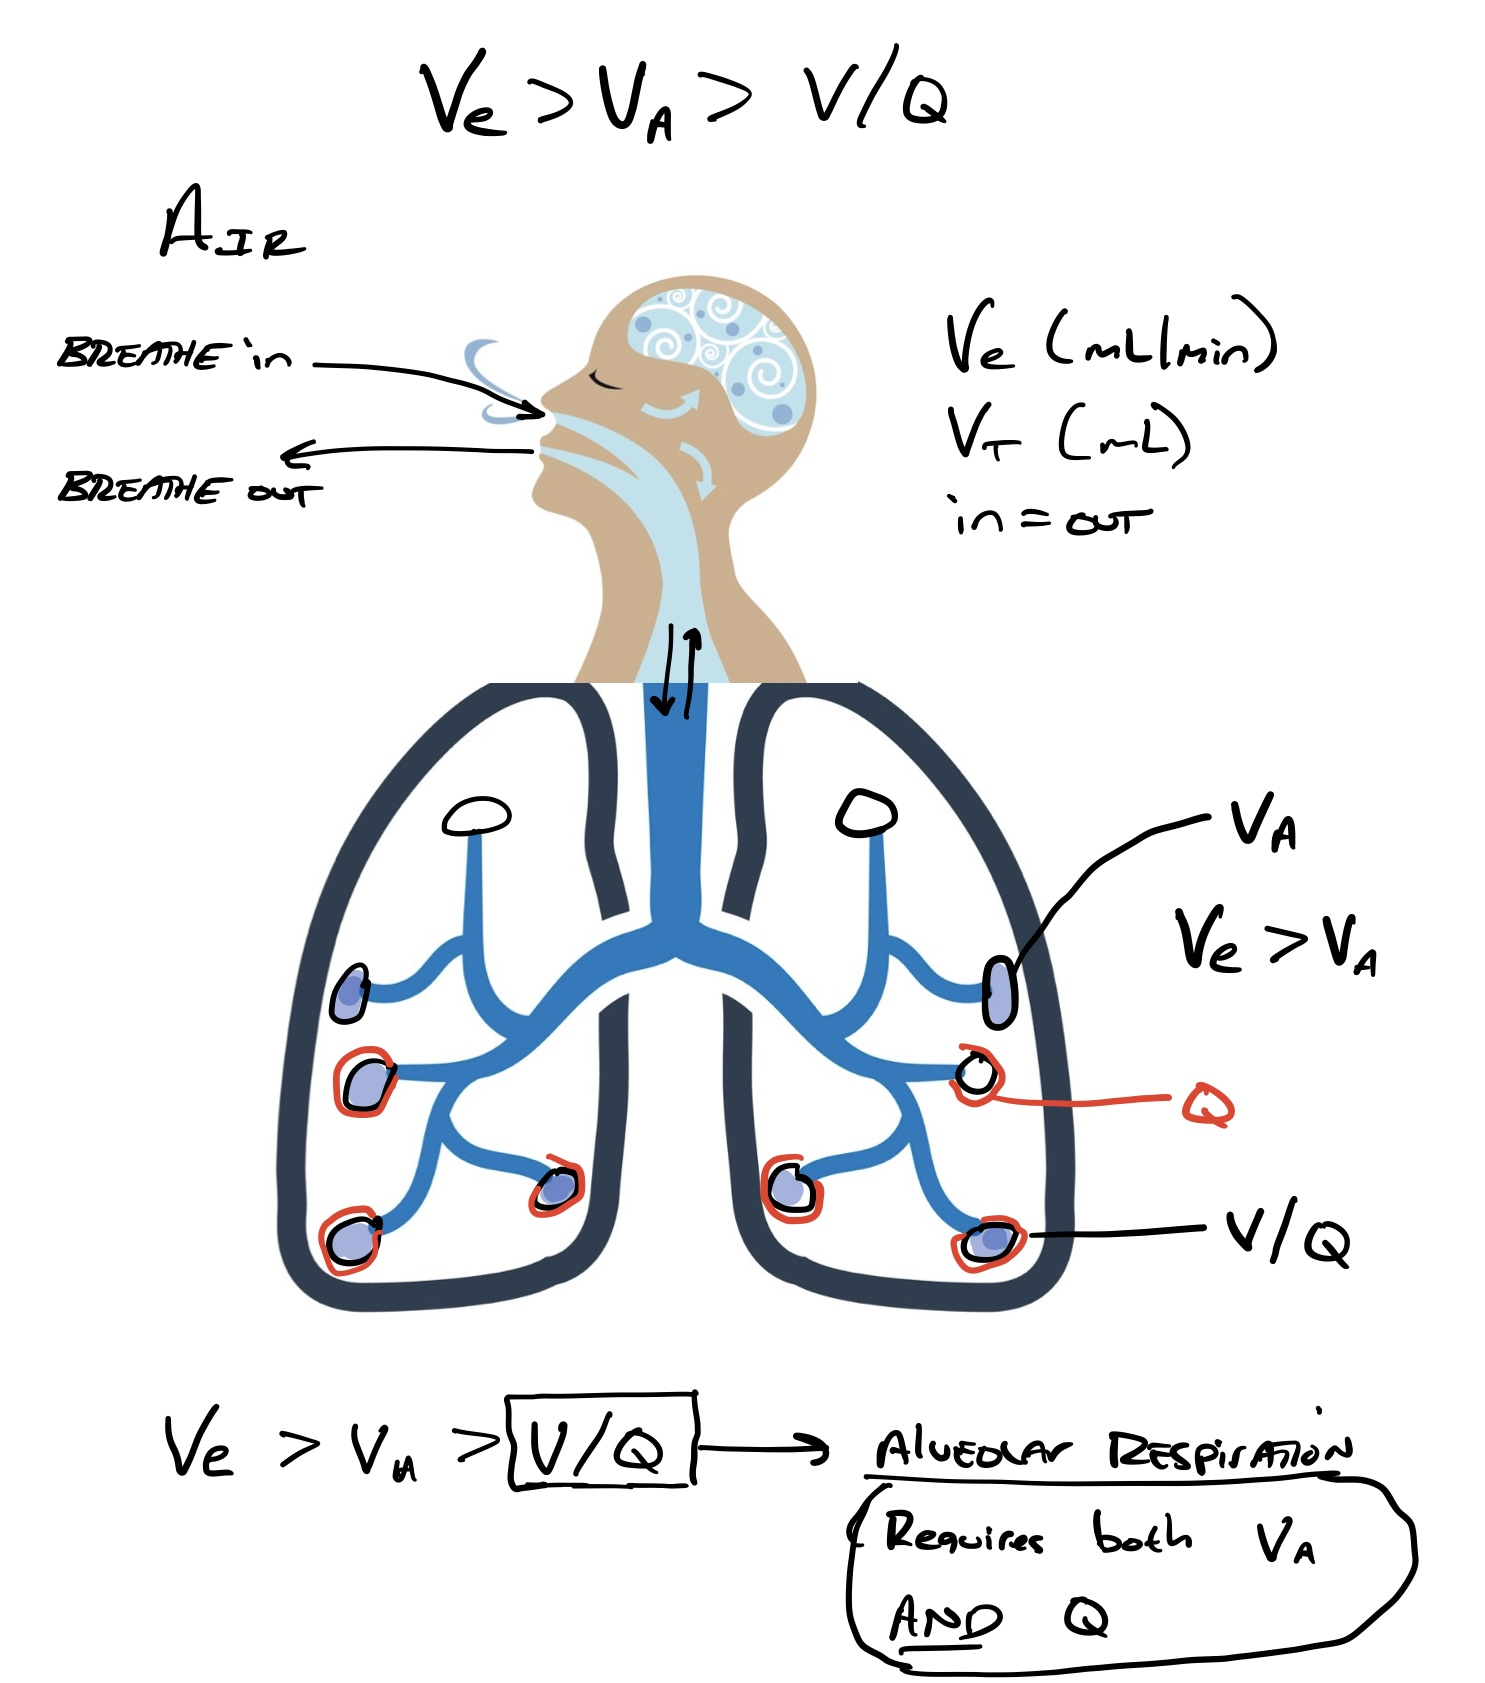
\includegraphics[width = 0.5\linewidth]{./figure/ve_va.jpg}
    \caption{Caption}
    \label{fig:ve_va.jpg}
\end{figure}

\paragraph{The importance of this concept} is that the alveolar respiration relies on the match between alveolar ventilation ($V_A$) and perfusion ($Q$). The consequences of all pulmonary (lung), and many cardiovascular, conditions ultimately rest on how they impact the ability to ventilate ($V_e$), the ability to turn as much $V_e$ into alveolar ventilation ($V_A$) as possible, or the ability to have as much $V_A$ perfusion as possible.

\subsection{Dead Space Ventilation ($V_D$}
Dead space ventilation that does not reach the alveoli (anatomical dead space), or that reaches the alveoli but does not receive perfusion (alveolar dead space). The combination of anatomical and alveolar dead space is called physiological dead space ($V_D$. To understand anatomical dead space ($VD_{ana}$) it is important to understand the structure and function of the airways.

\section{Airways}

The pathway of $O_2$ from the environment to the alveoli (or alveoli to the environment when considering $CO_2$) involves passage through a set of airways. It is important to recognize that only the alveoli are capable of gas exchange (diffusion, respiration). The difference between $V_e$ and $V_A$ starts with the airways.  

Figure \ref{fig:airways} includes the airways connecting the environment to the alveoli.

\begin{figure}[!h]
    \centering
    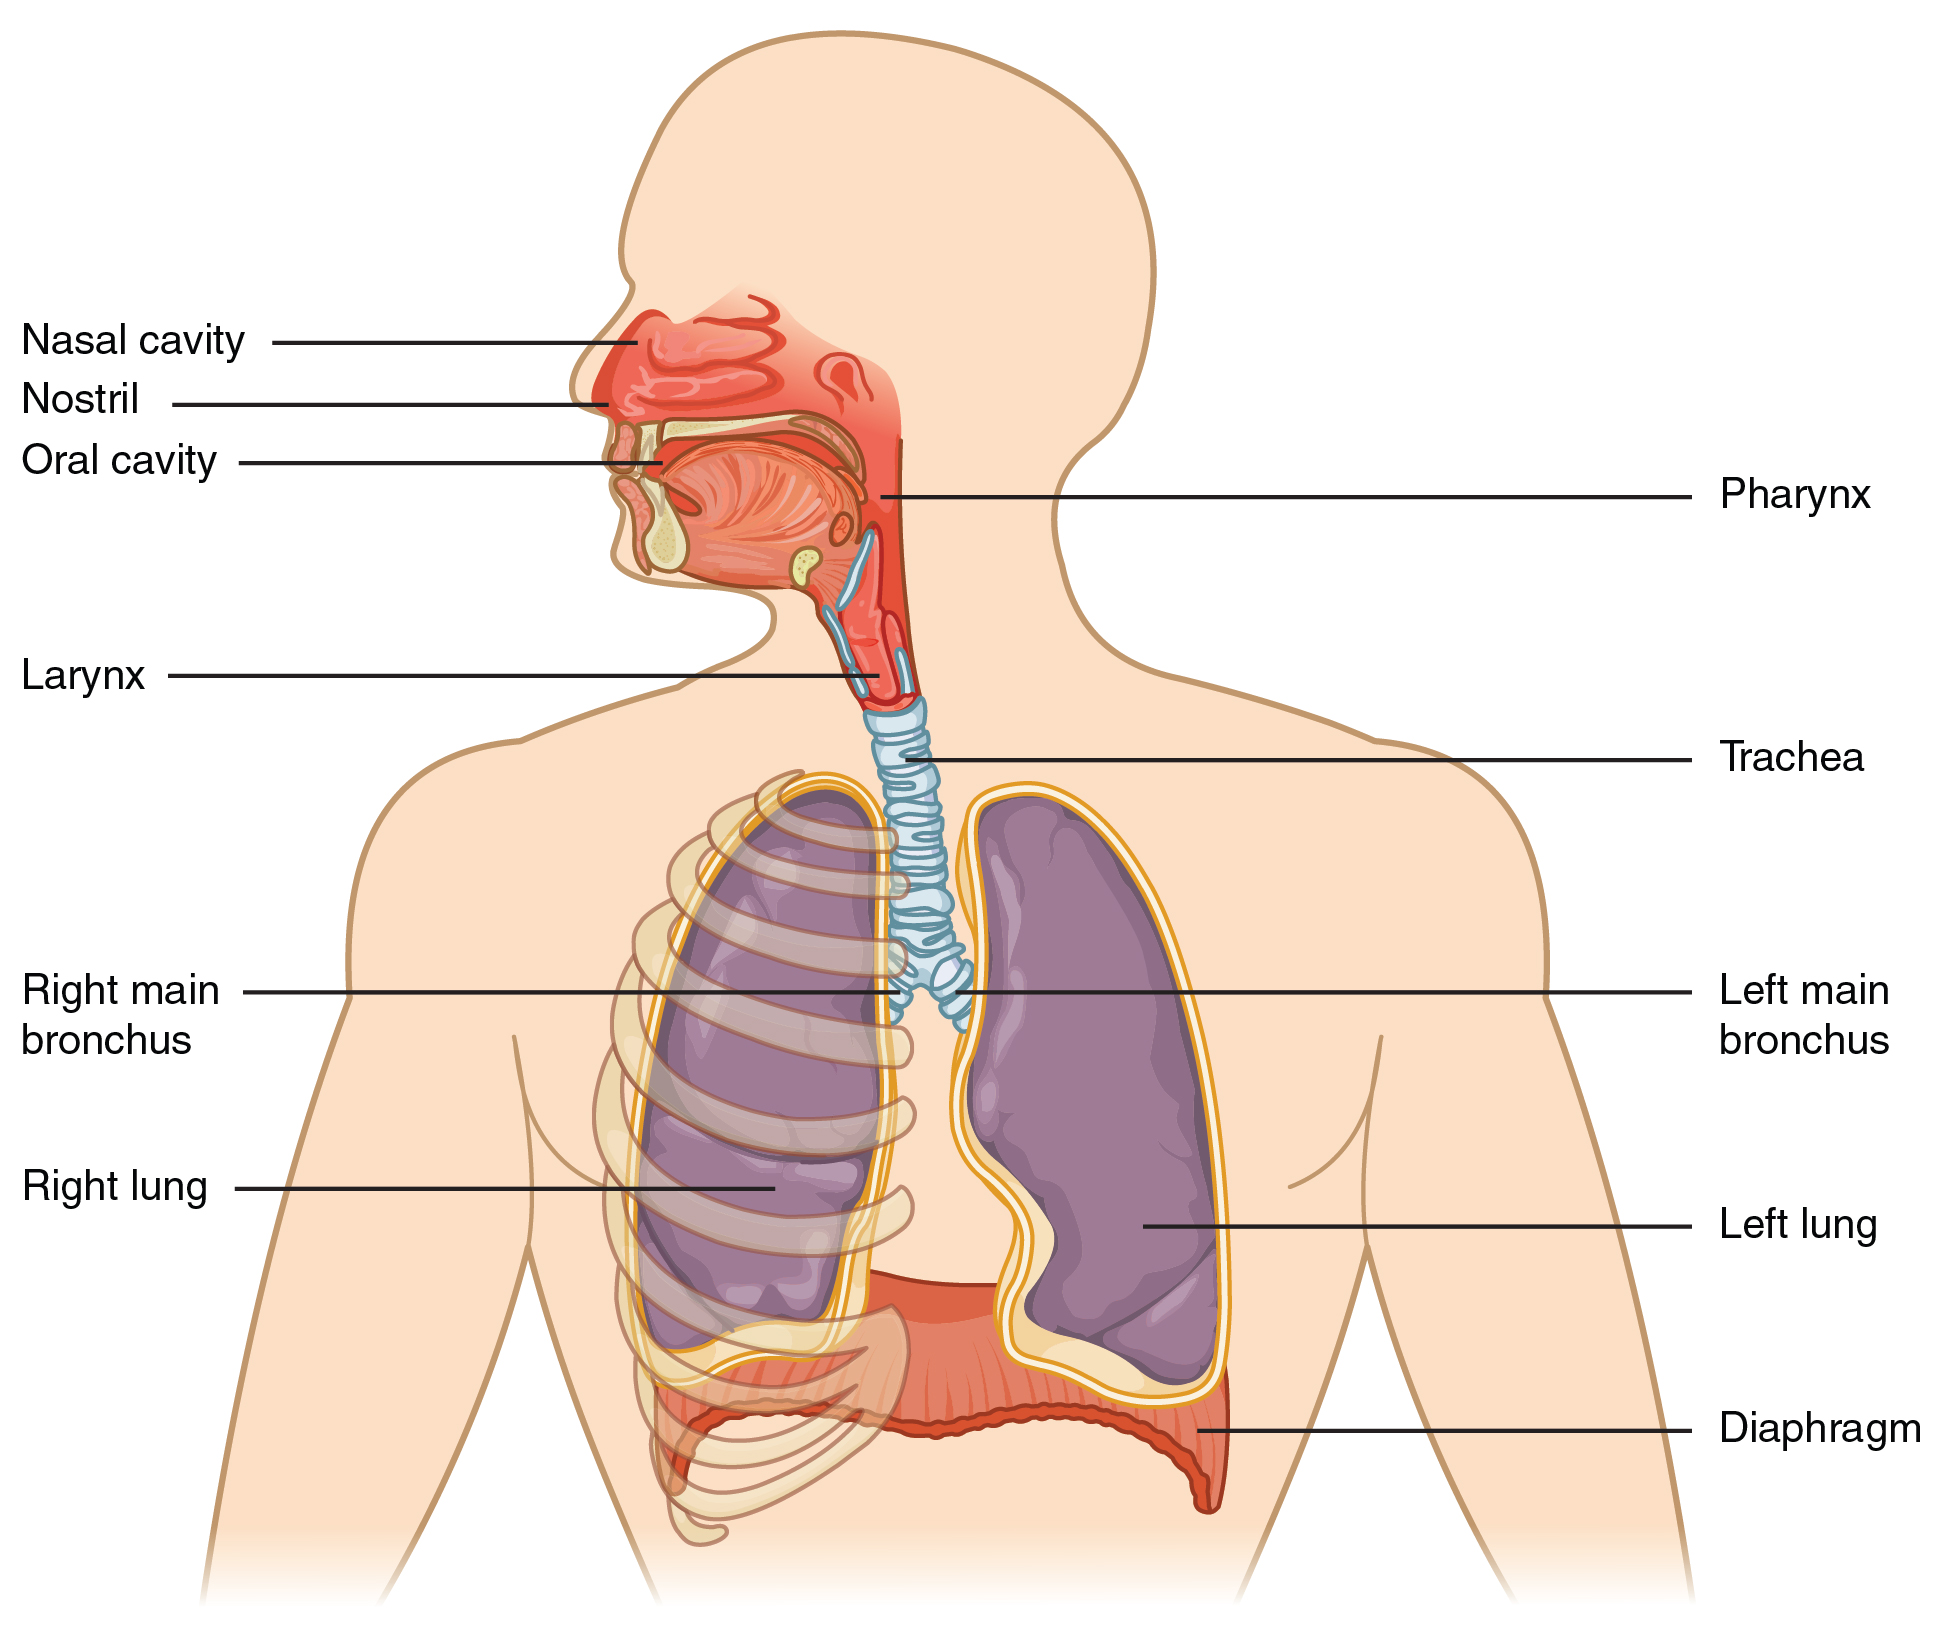
\includegraphics[width=1.0\linewidth]{./figure/airways.png}
    \caption{Passage to and from Alveoli}
    \label{fig:airways}
\end{figure}

\subsection{Anatomical Dead Space ($VD_{ana}$)}

Any air that enters the airways is part of $V_e$, but it is not part of $V_A$ unless it reaches an alveoli. For example, at the end of an inspiration the air remaining in the upper airways (nasal passages, the back of the throat, trachea) is part of $V_e$, but not part of $V_A$. The volume of air that is taken into the airways that does not reach the alveoli is referred to as anatomical dead space ($VD_{ana}$) and represents the conduction (non respiration) zone of the airways. $VD_{ana}$ is considered a fixed volume ($mL$). For example, if $VD_{ana} = 100 mL$, and 400 $mL$ is inspired with tidal volume ($V_T$), then 300 ($mL$) reaches alveoli ($V_A$). 

\paragraph{Question:}

Does $V_A (mL/min)$ change if $V_e (mL/min)$ stays the same but is achieved with different volume ($mL$) per breath at different breathing frequencies (respiratory rates)? Answer this by figuring out the $V_A (mL/min)$ and $V_e (mL/min)$ if $VD_{ana} = 100 mL$ when breathing 24 breaths per minute at 250 $mL/breath$; as compared to breathing 12 breathes per minutes at 500 $mL/breath$; as compared to breathing 6 breaths per minute at 1000 $mL/breath$. With each breathing pattern, $VD_{ana} = 100 mL$ since this is a fixed volume.

\subsection{Upper Airways}

The upper airways include the nasal passageways, the nasopharynx, the pharynx. Up to this point (the pharynx) the oral passages are also an option (but suboptimal) for breathing. The nasopharynx passes into the oropharynx which passes into the hypopharynx (laryngopharynx). At this point the epiglottis is the gatekeeper between the larynx (for air) and the esophagus (for food and drink).  The larynx includes the vocal cords and then continues into the trachea (beginning of the lower airways). 

Upper airway passages are lined with epithelial cells that include, in various locations, mucus production cells and cilia. Cilia are small cellular extensions that promote the movement of substances such as mucus across the membrane surface. Mucus and cilia in the airways are combined as a defense mechanism referred to as mucociliary activity. Together they promote the trapping of particles in mucus (including pathogens) and moving the mucus for removal through sneezing (nasopharynx), coughing (deeper than the nasopharynx), or swallowing (as an option when at the level of the hypopharynx near the epiglottis). 

\subsubsection{Bronchopulmonary Hygiene \& Airway Clearance}
Mucocilary activity is an important component of what is called bronchopulmonary hygiene (BPH), while sneezing and coughing are called airway clearance. Techniques to facilitate airway clearance are airway clearance techniques (ACT). BPH and ACT include several manual techniques within the physical therapy scope of practice.\footnotemark\footnotetext{Please don't tell me that "respiratory therapy" does this, of course they do. But that does not negate the fact that this is part of the PT scope of practice. If PTs did not do the things in their scope of practice that other professionals do, physical therapists would not do anything. Saying "respiratory therapy" does this - is like saying "massage therapists" do this about soft tissue mobilization; or that "chiropractors" do this about joint mobs/manipulations; or that "athletic trainers" or "OTs" do this about rehabilitation; or that "exercise physiologists" or "personal trainers" or "strength and conditioning specialists" do this about exercise prescriptions. Of course that is all true. Doing one thing is NOT what makes any of those professionals the professionals that they are, it is doing those things in context and the variety of things being done that makes each of these professions, including physical therapy. The PT uses BPH-ACT in in the plan of care for patients receiving PT, which will undoubtably include many other interventions based on client needs.} Just as increasing tissue extensibility through manual techniques may facilitate the range of motion necessary to move during therapeutic exercise to then maintain tissue extensibility; improving ventilation and respiration through manual techniques may facilitate the respiration necessary to move during exercise to then maintain respiration.  

\subsubsection{Nasal Passageways} are lined with epithelial cells rich in olfactory sensors (sense of smell) and goblet cells which are responsible for creating the mucus membrane. The passages include a set of turbinates that create turbulent flow of air through the passageways which is important for immunity, humidification, adding nitric oxide and the sense of smell. The turbulent flow of air encourages interaction between the air entering the the nasal passages and the cellular epithelial mucus membrane. Large particles (dust, many pathogens, allergens) never get past becoming stuck in the mucus of the nasal passage membranes, serving an important immune and protective function. Interaction with the nasal passage membrane also humidifies the air (adds water) and adds nitric oxide (NO). NO enhances local defense mechanisms via direct inhibition of pathogen growth and stimulation of mucociliary activity. NO from the nose and sinuses that is added to the air with every breath taken through the nose. NO reaches the alveoli in a more diluted form and enhances alveolar respiration by local vasodilation of pulmonary capillaries.

\subsubsection{Lower Airways}
The trachea is the airway that bridges the upper airways to the many airway divisions that will terminate in alveoli. The trachea is supported by large connective tissue rings that keep it open during wide fluctuations in thoracic pressures (coughing, sneezing, valsalva manuever). The trachea divides at the carina into two main bronchi (right and left) for the right and left lungs (respectively). 

Each bronchi splits into two branches for approximately 17 generations until ending with approximately 300,000 alveoli. The final branch of the bronchi is a bronchiole and is sometimes referred to as the respiratory bronchiole. The lower airways are also lined with epithelial cells that produce mucus and have cilia, and thus also have mucociliary activity that contributes to bronchopulmonary hygiene (BPH) and airway clearance. 

Similar to the artery to arteriole tree, each branch of the the bronchi to bronchiole tree gets progressively smaller, while the sum of space gets larger; and the influence of smooth muscle on the radius gets more important. For example, the main bronchi is larger than any single branch, but the branches, summed together, offer far more space than the main bronchi. As the branches get smaller with each generation of splitting the walls get thinner and the influence of smooth muscle on the walls gets more influential. Most bronchodilation and bronchoconstriction occurs in the smaller bronchioles than in the larger bronchi.

\paragraph{Bronchodilation \& bronchoconstriction} are regulated by sympathetic nervous system innervation and endocrine function (circulating epinephrine and norepinephrine). Sympathetic activity has the opposite effect on bronchioles as they do on arterioles. Increased symphathetic activity bronchodilates and decreased sympathetic activity bronchoconstricts. Conditions that create bronchoconstriction, such as asthma, are therefore commonly treated with adrenergic agonist inhalers (inhaled medication).  

\section{Volumes \& Capacities}

Ventilatory volumes and capacities are depicted in Figure \ref{fig:ventilation_volumes}. Capacities are combinations of volumes.

\begin{figure}[!h]
    \centering
    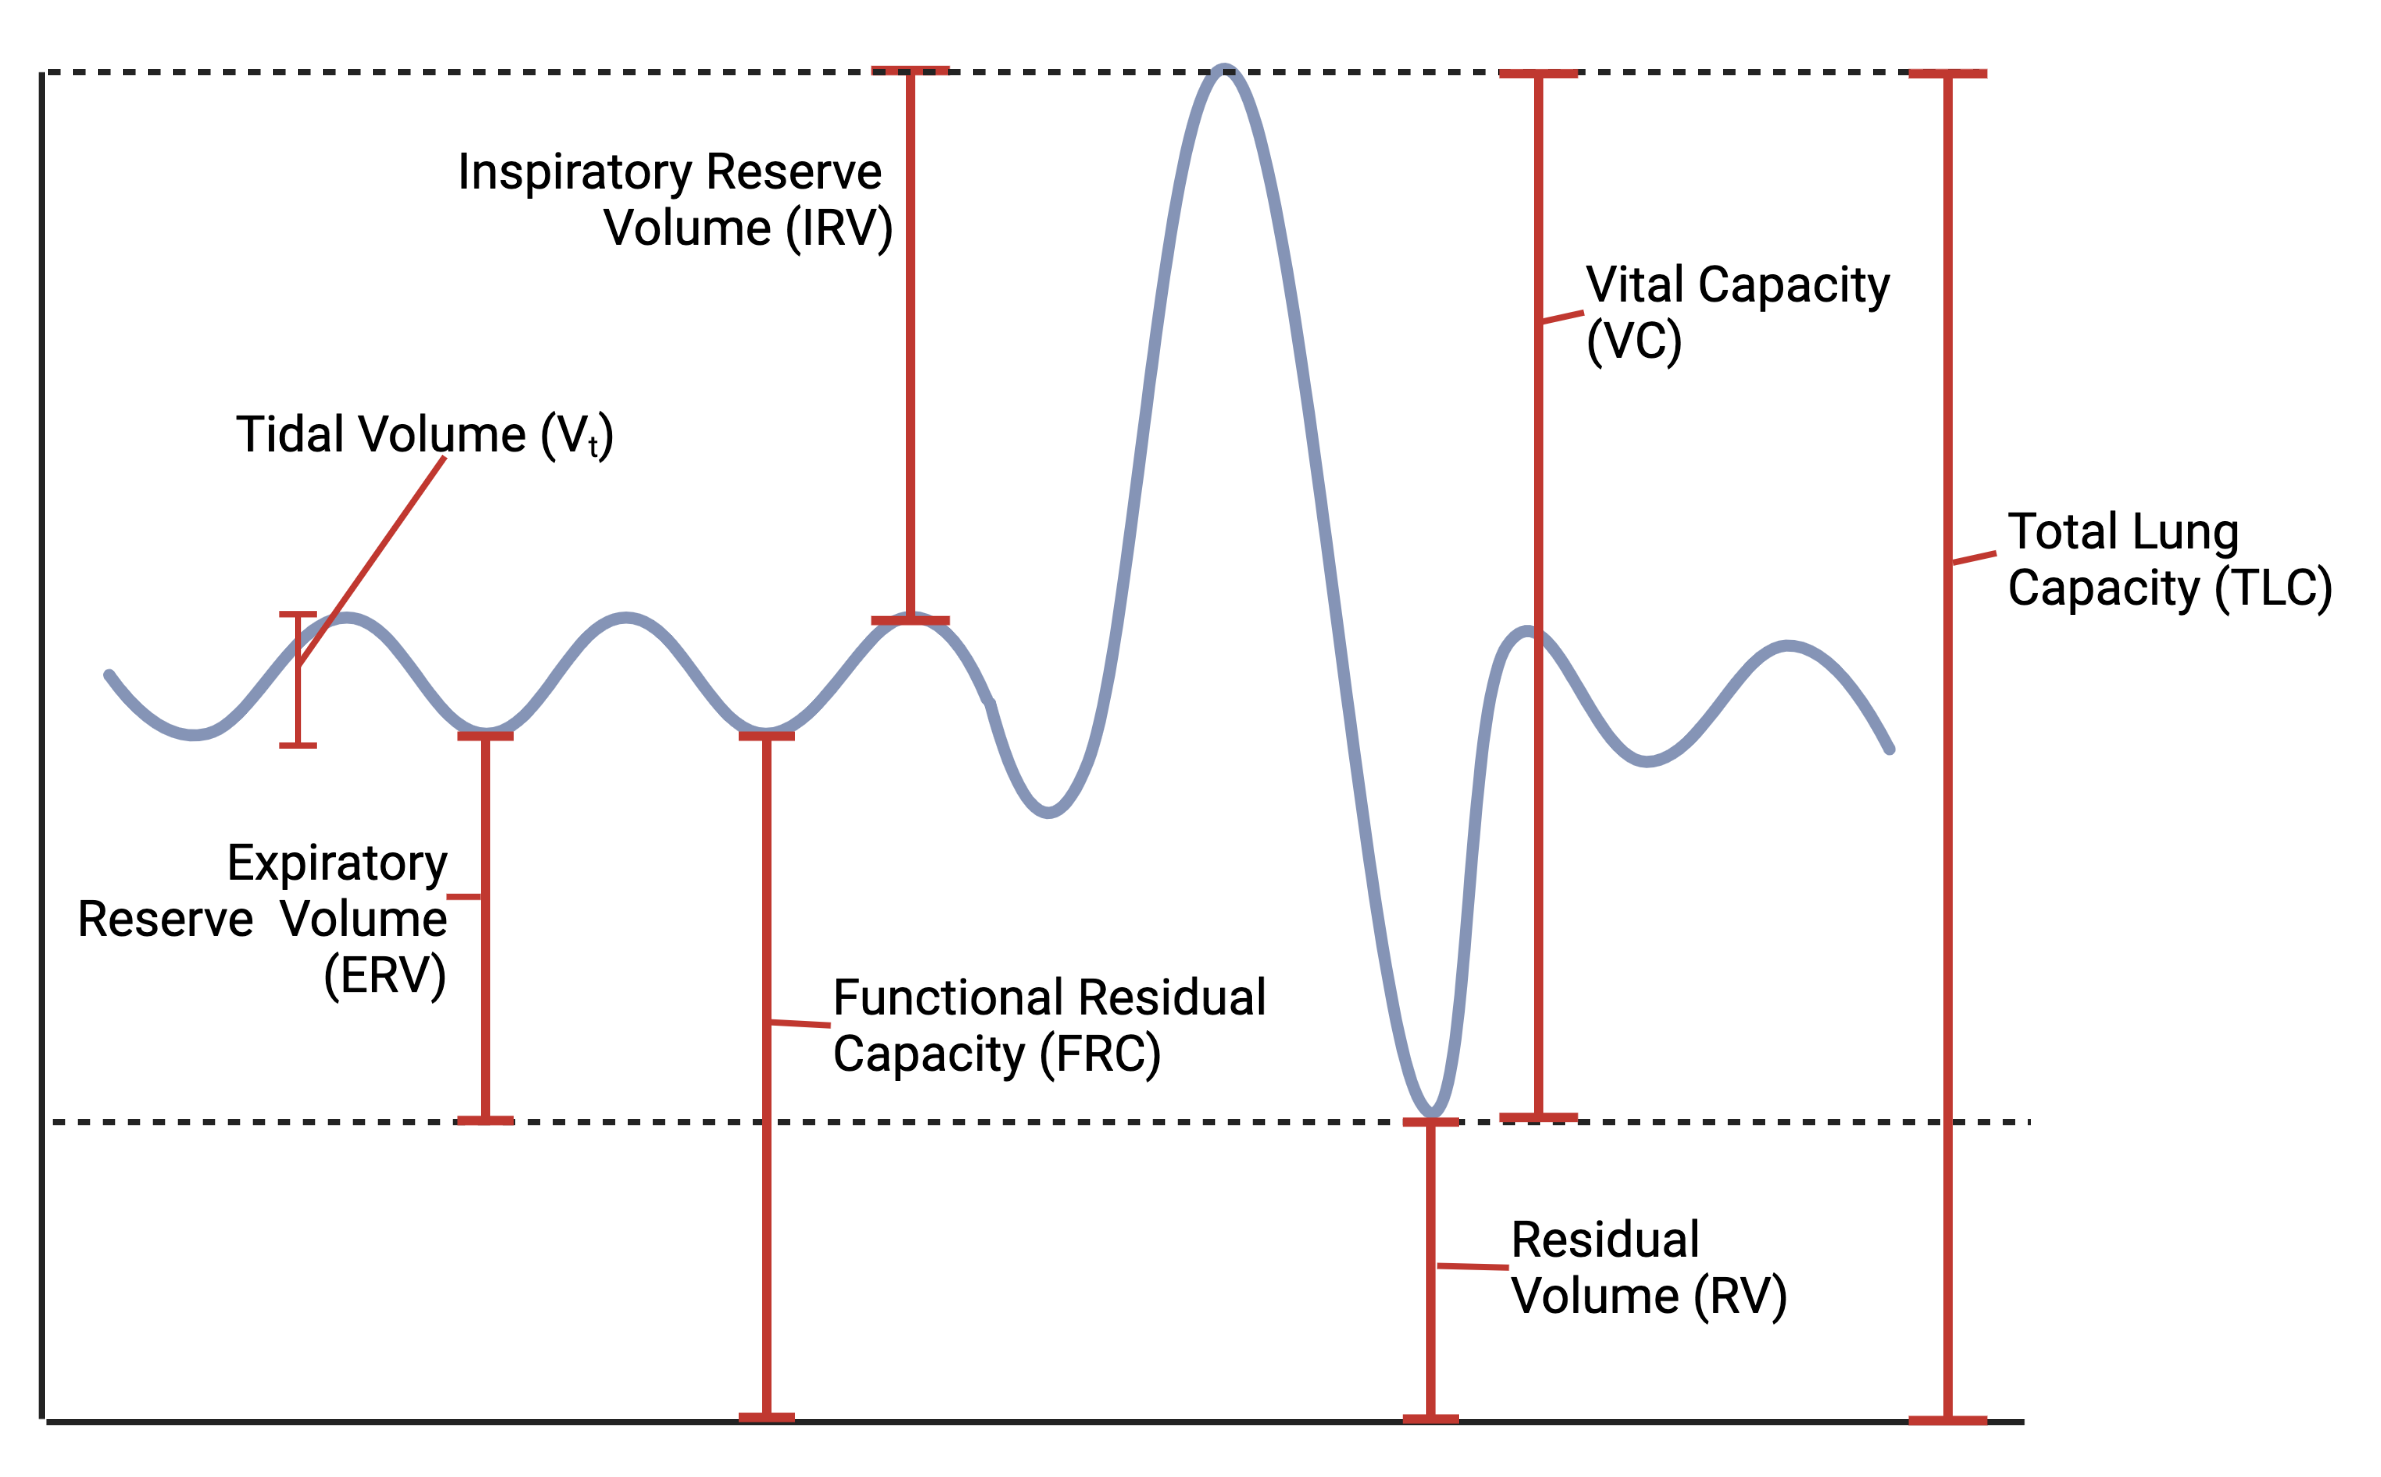
\includegraphics[width=1.0 \linewidth]{./figure/ventilation_volumes.png}
    \caption{Ventilatory Volumes \& Capacities}
    \label{fig:ventilation_volumes}
\end{figure}

\begin{itemize}
    \item Tidal Volume ($V_t$): Volume of breathing. $V_T$ varies in order to change ventilation $V_e$, for the purpose of changing $V_A$ to meet the needs of alveolar respiration as it maintains $Pa_CO_2$ and $P_aO_2$; or adjusts $Pa_CO_2$ as part of acid base balance regulation.
    \item Inspiratory Reserve Volume ($IRV$) is the volume that can be inhaled after a normal $V_t$ inspiration
    \item Expiratory Reserve Volume ($ERV$) is the volume that can be exhaled after the end of a normal $V_t$ expiration
    \item Residual Volume ($RV$) is the volume that cannot be exhaled
    \item Vital Capacity ($VC$) is $V_t + ERV + IRV$, it is the largest volume that can be breathed in after a complete exhalation, or out after a complete inspiration
    \item Functional Residual Capacity ($FRC$) is $ERV + RV$, it is the volume of air remaining in the lungs after a normal expiration
    \item Total Lung Capacity ($TLC$) is $IRV + V_t + ERV + RV$, it total capacity for air in the lungs
\end{itemize}

% Ended here


\subsection{Mechanics}

Diaphragm as a muscle


Inspiratory muscles - primarily diaphragm (phrenic nerve, C1-3); diaphragm tensions pulls the thoracic cavity down (central tendon extends down to it's attachments); and it pulls up on the lower ribs


internal intercostals, any muscle that can expand the chest wall (spinal extensors, scalenes, sternocleomastoid)

Expiratory muscles - only needed during exhalation at rates greater than resting tidal breathing, or forced expiratory manuevers such as sneezing, coughing; external intercostals; abdominal muscles (including transverse abdominus, internal and external obliques, rectus abdominus)

Rib movements


\subsection{Pressures}





\section{Ventilation - Perfusion Matching}

\begin{itemize}
       \item Anatomical dead space is air ventilated but that does not make it into alveoli. Anatomical dead space = $V_e - V_A$
    \item Physiological dead space occurs in alveoli that receive ventilation but do not receive alveolar circulation
    \item Dead space ventilation ($V_{DS}$) is the sum of anatomical and physiological dead space
\end{itemize}


Chapter \ref{chp:alveolar_oxygen} on Ventilation considers the concept of ventilation - perfusion $\dot{V}/\dot{Q}$ matching, the impact of body position on $\dot{V}/\dot{Q}$ matching zones, and the impact of $\dot{V}/\dot{Q}$ matching on the $P_AO_2-P_aO_2$ gradient, otherwise known as the A-a gradient.
\subsection{Perfusion Zones}
$\dot{V}/\dot{Q}$

requires a continuous exchange (refresh) of air in the alveoli with the environment known as alveolar ventilation ($V_A$). $V_A$ needs to matched with alveolar capillary blood flow. $V_A$ requires ventilation (breathing); and alveolar capillary blood flow requires the distribution of pulmonary circulation ($Q$) to ventilated alveoli. 


\subsection{A-a Gradient}


\section{Regulation}

Automatic but voluntary control - we breath without thinking about it, but we can think about it and control it (like posture and gait)

%The regulation of blood $O_2$ and $CO_2$ includes monitoring these values with chemoreceptors, but the efferent (action) side of these regulatory pathways include variations in ventilation.


\section{Practice Connections}

\subsection{Nose vs. mouth breathing}

\subsection{Pulmonary Function Tests - Forced Expiratory Manuever}

\subsection{Ventilatory Insufficiency Patterns}

\printbibliography[heading=subbibintoc]